\section{Metode Penelitian}
\begin{frame}
\frametitle{Metode Penelitian}
\begin{block}{Tahapan Penelitian}
\begin{figure}[H]
\centering
%Definisi
\tikzstyle{kotak} = [rectangle, minimum height=2cm, text width=3cm, text centered, draw=black, fill=blue!30]
\tikzstyle{garis} = [thick,->,>=stealth]
%Gambar
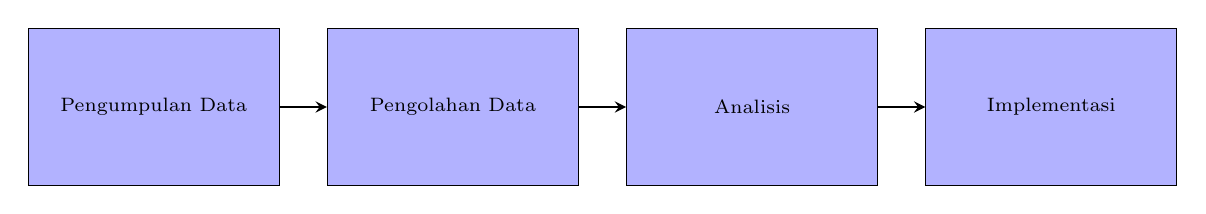
\begin{tikzpicture}
\scriptsize
\onslide<1-> \node (1) [kotak] {Pengumpulan Data};
\onslide<2-> \node (2) [kotak, right of=1, xshift=+2.8cm]{Pengolahan Data};
\onslide<3-> \node (3) [kotak, right of=2, xshift=+2.8cm]{Analisis};
\onslide<4-> \node (4) [kotak, right of=3, xshift=+2.8cm]{Implementasi};

\onslide<1-> \draw [garis] (1) -- (2);
\onslide<2-> \draw [garis] (2) -- (3);
\onslide<3-> \draw [garis] (3) -- (4);
\end{tikzpicture}
\end{figure}
\end{block}

\begin{block}<5->{Data Penelitian}
Dalam penelitian ini data yang digunakan adalah nama dan koordinat lokasi dari seluruh SMA di Kabupaten Probolinggo yang dikumpulkan dari:

\begin{enumerate}
\item \url{https://referensi.data.kemdikbud.go.id/} (Daftar Nama Sekolah di Kabupaten Probolinggo)
\item \url{https://earth.google.com/} (Koordinat lokasi sekolah)
\end{enumerate}
\end{block}
\end{frame}